\documentclass[conference]{IEEEtran}
\IEEEoverridecommandlockouts
% The preceding line is only needed to identify funding in the first footnote. If that is unneeded, please comment it out.
\usepackage{cite}
\usepackage{amsmath,amssymb,amsfonts,mathtools}
\usepackage{algorithmic}
\usepackage{graphicx}
\usepackage{textcomp}
\usepackage{xcolor}
\usepackage{indentfirst}
\usepackage{hyperref}
\hypersetup{
    colorlinks=true,
    linkcolor=blue,
    filecolor=magenta,      
    urlcolor=cyan,
}
\def\BibTeX{{\rm B\kern-.05em{\sc i\kern-.025em b}\kern-.08em
    T\kern-.1667em\lower.7ex\hbox{E}\kern-.125emX}}
\begin{document}

\title{To check whether an element X is present in an array or not using Divide and Conquer Algorithm\\
{\footnotesize \textsuperscript {} Indian Institute of Information Technology, Allahabad}
}

\author{\IEEEauthorblockN{Aditya Aggarwal}
\IEEEauthorblockA{\textit{iit2019210@iiita.ac.in}}
\and
\IEEEauthorblockN{Divy Agrawal}
\IEEEauthorblockA{\textit{iit2019211@iiita.ac.in}}
\and
\IEEEauthorblockN{Aman Rubey}
\IEEEauthorblockA{\textit{iit2019212@iiita.ac.in}}
}

\maketitle

\begin{abstract}
 In this paper we have devised an algorithm to find an element X in an array of given elements solely using the concept of divide and conquer. Also in the later part of the paper we have discussed the space and time complexity of the devised algorithm.
\end{abstract}

\begin{IEEEkeywords}
Algorithm, Divide and Conquer, Searching, complexity
\end{IEEEkeywords}

\section{Introduction}
Divide and conquer algorithm is an efficient algorithm that decompose a given problem into small sub-problems recursively until it is relatively easier to solve those small sub-problems. Then the solution to the original problem is computed by combining the solutions to the sub-problems. Implementation of this algorithm could be seen in sorting algorithms such as merge-sort and quick-sort. 

\section{Algorithm Design}
We have taken elements (Integer) as input from user and stored them in a vector. We will be using this vector to check whether an element X is present in this vector.

An important concept used in this algorithm is that if vector contains a singleton element only and if this element is equal to the required element X the answer would be true else it would be false.
% \vspace{5pt}
% \hrule height 0.4pt depth 1pt width 250pt \relax
% \vspace{5pt}
% jfsdkfjsfsmlfmjsfjksfs
% \\
% \hrule height 0.4pt depth 1pt width 250pt \relax

\begin{itemize}
\item Here the main problem is to check whether an element is present in a vector or not.
\item This main problem could be divided into two sub-problems by dividing this initial vector (parent vector) into two vectors (child vectors) of approximately same size and checking whether the required element is present in these two vectors formed(child vectors).
\item We will divide these new sub-vectors formed until the new vectors comprise of singleton element only.
\item As discussed earlier in this section, answer for these vectors comprising of single elements will be either true or false depending on whether this single element is equal to required element or not.
\item Suppose, we know that whether the required element X is present in two vectors or not. Then the answer to the problem-vector comprising of the elements of both the vectors simply depends upon the answer for the two child vectors.
\begin{itemize}
    \item If element is present in either or in both of the child vectors then the element will be present in the parent vector comprising of these two child vectors.
    \item If element is not present in both of the child vectors then the element will not be present in the parent vector comprising of these two child vectors.
\end{itemize}
\item Similarly, we will be checking whether the required element is present in all of the sub-vectors (child vectors) previously created or not. And, this then would be used to compute whether element is present in the parent vector or not.
\end{itemize}

These 6 steps of the algorithm would become more clear by the following example:
\begin{itemize}
\item Consider a vector V.
\begin{center}
    V $\equiv$ \{34, 4, 56, 999\}
\end{center}
We want to check whether the element X=999 is present or not in this vector using divide and conquer.
\item We will now divide this vector V into two sub-vectors V\textsubscript{1} and V\textsubscript{2} which is equivalent to dividing problem-1 into two sub-problems problem-1a and problem-1b.
\begin{center}
    V\textsubscript{1} $\equiv$ \{34, 4\}\\
    V\textsubscript{2} $\equiv$ \{56, 999\}
\end{center}
Now we will check whether X is present in these sub-problems formed or not.
\item We will now divide vector V\textsubscript{1} into two sub-vectors V\textsubscript{11} and V\textsubscript{12} which is equivalent to dividing problem-1a further into two sub-problems problem-1a1 and problem-1a2.
\begin{center}
    V\textsubscript{11} $\equiv$ \{34\}\\
    V\textsubscript{12} $\equiv$ \{4\}
\end{center}
Similarly, we will now divide vector V\textsubscript{2} into two sub-vectors V\textsubscript{21} and V\textsubscript{22} which is equivalent to dividing problem-1b further into two sub-problems problem-1b1 and problem-1b2.
\begin{center}
    V\textsubscript{11} $\equiv$ \{56\}\\
    V\textsubscript{12} $\equiv$ \{999\}
\end{center}
Now we will check whether X is present in these sub-problems formed or not.
\item As discussed earlier, solutions to the sub-problems problem-1a1, problem-1a2, problem-1b1, problem-1b2 will be either true or false depending upon whether these singleton element is equal to required element or not.\\ Therefore, solution to these sub-problems will be:
\begin{enumerate}
    \setlength{\itemindent}{1em}
    \item Problem-1a1 is false as 34 is not equal to 999.
    \item Problem-1a2 is false as 4 is not equal to 999.
    \item Problem-1b1 is false as 56 is not equal to 999.
    \item Problem-1b2 is true as 999 is equal to 999.
\end{enumerate}
This now will be used to compute solution for the sub-problems problem-1a and problem-1b.
\item Solution to the sub-problem problem-1a will be false as solution to the sub-problems problem-1a1 and problem-1a2 is false. This means that 999 is not present in the vector V\textsubscript{1} which is true.\\
Solution to the sub-problem problem-1b will be true as solution to the sub-problem problem-1b2 is true despite of solution to problem-1b1 is false. This means that 999 is present in the vector V\textsubscript{2} which is true.\\
Therefore, solution to these sub-problems will be:
\begin{enumerate}
    \setlength{\itemindent}{1em}
    \item Problem-1a is false.
    \item Problem-1b is true.
\end{enumerate}
This now will be used to compute solution for the main-problem, problem-1.
\item Solution to the main-problem problem-1 will be true as solution to the sub-problem problem-1b is true despite of solution to problem-1a is false. This means that 999 is present in the vector V which is true.\\Thus, the required element 999 is present in the vector V (main-problem).
\end{itemize}

These above 6 steps of the example clearly show how we have used divide and conquer algorithm i.e., we firstly divided the main-problem into small sub-problems until they we were able to solve them directly. Then we computed the answer for these sub-problems and used these answers to compute answer for the main-problem.
\\
\section{Pseudo Code}
\vspace{5pt}
\hrule height 0.4pt depth 1pt width 250pt \relax
\vspace{5pt}
\textbf{Algorithm using Divide and Conquer}
\vspace{5pt}
\hrule height 0.4pt depth 1pt width 250pt \relax
\vspace{5pt}
\textbf{\textit{Global Variables:}}\\
\hspace*{6mm} vector\langle int\rangle v;\\
\hspace*{7mm} int\ n;\\
\hspace*{7mm} int\ x;\\
\\
\hspace*{4mm}\textbf{\textit{function}}\ main()\\
\hspace*{7mm}Get\ n;\\
\hspace*{7mm}Get\ n\ elements\ and\ store\ them\ in\ a\ vector;\\
\hspace*{7mm}solution\ \leftarrow\ solve(0,n-1);\\
\hspace*{7mm}print\ solution;\\
\hspace*{7mm}return\ 0;\\
\\
\hspace*{4mm}\textbf{\textit{function}}\ solve(low, high)\\
\hspace*{7mm}if\ low\ ==\ high\ then\\
\hspace*{10mm}if\ v[low]\ ==\ x\ then\\
\hspace*{13mm}return\ true;\\
\hspace*{10mm}else\\
\hspace*{13mm}return\ false\\
\hspace*{7mm}mid\ \leftarrow\ low+(high-low)/2\\
\hspace*{7mm}return\ (solve(low,\ mid)\ OR\ solve(mid+1,\ high))\\
\vspace{5pt}
\hrule height 0.4pt depth 1pt width 250pt \relax
\vspace{5pt}
\section{Complexity Analysis}
In the next two sub-sections we analyse the time and space complexity of algorithm we devised for the given problem.
\subsection{Time-Complexity}
Let N denote the number of elements in the vector in which we have to check whether the required element is present or not.\\
\begin{figure}[htbp]
\centerline{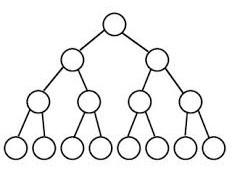
\includegraphics{image20.jpg}}
\caption{Problem Dividing in Divide and Conquer}
\label{fig}
\end{figure}\\

Taking  the reference of the above tree, where root node denotes  the main-problem and rest nodes denote the sub-problems formed from the main-problem. Suppose if the time-complexity of the problem consisting of N elements is T(N) then the time-complexity of sub-problems of this problem will be T(N/2) approximately and let time-complexity for executing rest statements be C\textsubscript{1}.\\
Then,\\
\begin{equation}
    T(N) = 2T(N/2) + C\textsubscript{1}
\end{equation}
which is equivalent to,
\begin{equation}
    T(N) = 2T(N/2) + \Theta(1)
\end{equation}
Therefore, upon applying master’s theorem we get,
\begin{equation}
    T(N) = O(N)
\end{equation}
\subsection{Auxiliary Space-Complexity}
Let N denote the number of elements in the vector in which we have to check whether the required element is present or not.

The function solve(low,high) is being called approximately 2N-1 times that is O(N) times and each time when it is called 3 variables of size 4 bytes is created.
Therefore, Auxiliary Space-Complexity will be,
\begin{equation}
    T(N) = O(N)
\end{equation}
\section{Theortical complexity analysis}
\begin{figure}[htbp]
\centerline{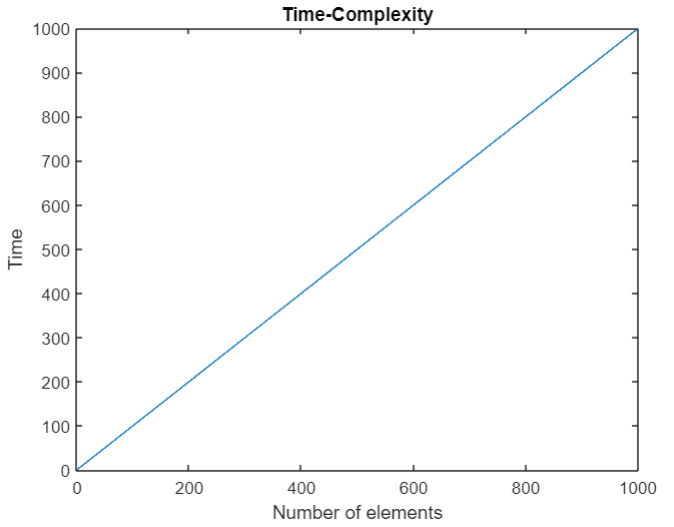
\includegraphics[width=9cm]{Time.png}}
\caption{Time–Complexity Graph (O(N))}
\label{fig}
\end{figure}
\begin{figure}[htbp]
\centerline{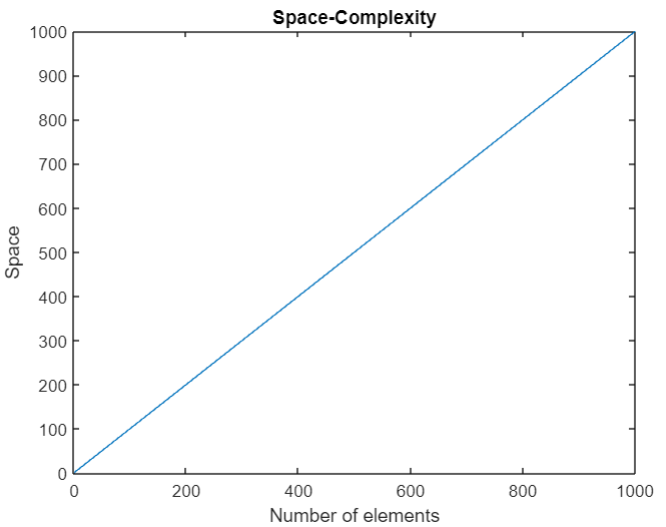
\includegraphics[width=9cm]{Space.png}}
\caption{Auxiliary Space–Complexity Graph (O(N))}
\label{fig}
\end{figure}
\section{Advantages Against Linear uni-processor Search}
\begin{enumerate}
    \item \ \ \ In the computer systems containing a single processor the execution of processes tends to be slow as a single process hogs the CPU till it's cycle is complete or execution of the process stops. So, OS generally implements multi-threading by itself at the software level without kernel knowing about it.\\

\ \ \ \ So in a Linear Uni-processor Search, the process of checking whether the element is present or not will be taking several CPU cycles before the we finally get the answer. In this the whole process we be running on a single main thread because of which it will become slow as the number of elements to search from increases.\\

\ \ \ \ But in Divide and Conquer Algorithm the main-task is divided into sub-tasks which are completely independent of each other. So, these independent sub-tasks could be executed using threads which are basically light-weight processes needing relatively less context switching time then that required for context switching of a process. These, solution to the sub-problems executed using threads could be used to compute the solution to other sub-problems depending upon these on a separate thread.\\

\ \ \ \ Because of this, when the number of inputs becomes very large Divide and Conquer Algorithm executes faster than Linear Uni-processor Search despite of the fact that both the algorithms have same time complexity. When the number of inputs are low the time of execution is same for both.\\
\item \ \ \ Another advantage of Divide and Conquer Algorithm is the use of memory caches efficiently as when the sub problems becomes very simple, they can be solved within the cache, without having to access the slower main memory(Cache is second fastest accessible memory after Registers), which saves a lot of time and makes the algorithm more efficient. And in some cases, it can even produce more precise outcomes in computations with rounded arithmetic than iterative methods would.
\end{enumerate}

\section{Conclusion}
Therefore, using the concept of divide and conquer we have devised an algorithm to check whether an element is present in a vector of elements or not. The time complexity of the above devised algorithm is O(N) where as auxiliary space complexity is O(N) where N is number of elements given by the user.\\
\begin{thebibliography}{00}
\bibitem{b1}Introduction to Algorithms 3rd Edition by Clifford Stein, Thomas H. Cormen, Charles E. Leiserson, Ronald L. Rivest
\bibitem{b2} Algorithm Design by J Kleinberg and E Tardos
\bibitem{b3} Abraham Silberschatz Peter B. Galvin and Greg Gagne, Operating System Concepts, Wiley 8th Edition, 2008
\bibitem{b4} \href{https://en.wikipedia.org/wiki/Divide-and-conquer_algorithm}{Divide and Conquer}
\bibitem{b5}\href{https://stackoverflow.com/questions/11032015/how-to-find-time-complexity-of-an-algorithm}{Complexity Analysis}
\bibitem{b6}\href{http://www.csun.edu/~mam78887/MAMANLEY.pdf}{Divide and Conquer Paradigm}
\end{thebibliography}
\end{document}